\chapter{Bausteinsicht}

Um ein besseres Verständnis über die Struktur des Systems zu bekommen, nutzen wir die Bausteinsicht. Sie hilft dabei ein gemeinsames Verständnis des Systems innerhalb des Teams zu bekommen.
Die zur Zerlegung benutzte Dekompistionsstrategie ist funktional. 

\section{Bausteinsicht Level 1}
 

\begin{figure}[h] % [h] = here
    \centering
    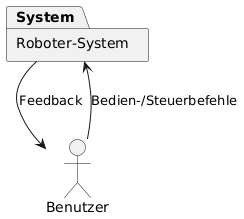
\includegraphics[width=0.6\textwidth]{diagrams/bausteinsicht_lvl_1_system_name_change.png}
    \caption{Bausteinsicht Level 1}
\end{figure}

\begin{table}[h!]
\centering
\begin{tabular}{|p{4cm}|p{9cm}|}
\hline
\textbf{Komponente} & \textbf{Beschreibung} \\ \hline
Robotic System & Gesamtsystem, das alle internen Steuer-, Safety- und Kommunikations­funktionen kapselt. Empfängt Bedien-/Steuerbefehle vom Benutzer, verarbeitet sie und liefert Feedback. \\ \hline
\end{tabular}
\caption{Bausteinsicht Level 1}
\label{tab:lvl1}
\end{table}

\newpage
\section{Bausteinsicht Level 2}
\begin{figure}[h] % [h] = here
    \centering
    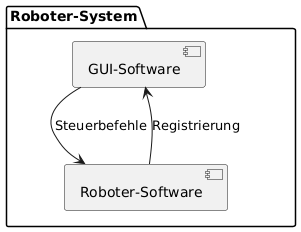
\includegraphics[width=0.6\textwidth]{diagrams/baustein_lvl_2.png}
    \caption{Bausteinsicht Level 2}
\end{figure}

\begin{table}[h!]
\centering
\begin{tabular}{|p{4cm}|p{9cm}|}
\hline
\textbf{Komponente} & \textbf{Beschreibung} \\ \hline
GUI-Software (ITS) & Bietet die Benutzeroberfläche, nimmt Steuerbefehle entgegen, zeigt den Zustand des ausgewählten Roboters an und leitet Befehle an die Roboter-Software weiter. \\ \hline
Roboter-Software (RS) & Führt Bewegungs- und Greifbefehle aus, steuert Hardware, registriert sich bei der GUI-Software und sendet Status­meldungen zurück. \\ \hline
\end{tabular}
\caption{Bausteinsicht Level 2}
\label{tab:lvl2}
\end{table}
\newpage

\section{Bausteinsicht Level 3}
\begin{figure}[h] % [h] = here
    \centering
    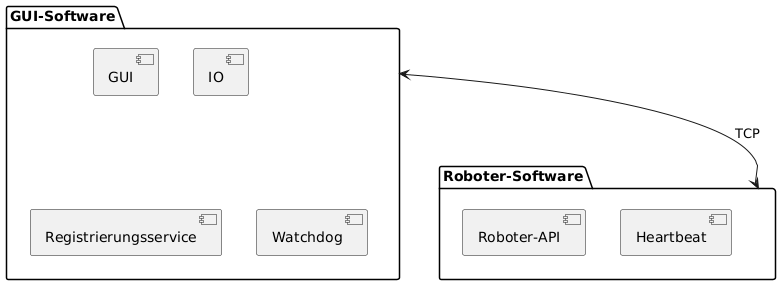
\includegraphics[width=0.6\textwidth]{diagrams/baustein_lvl_3.png}
    \caption{Bausteinsicht Level 3}
\end{figure}

\begin{table}[h!]
\centering
\begin{tabular}{|p{4cm}|p{9cm}|}
\hline
\textbf{Komponente} & \textbf{Beschreibung} \\ \hline
GUI & Frontend zur Eingabe von Befehlen und Anzeige von Status-/Fehler­meldungen. \\ \hline
IO  & Schnittstelle für Ein-/Ausgabe­geräte; leitet Steuerbefehle an die Roboter-API und empfängt Rückmeldungen. \\ \hline
Registrierungsservice & Authentifiziert und registriert Roboter-Software-Instanzen bei der GUI-Software. \\ \hline
Watchdog & Überwacht Laufzeit- und Funktions­fähigkeit der GUI-Software; löst Neustarts bei Fehlern aus. \\ \hline
Roboter-API & Abstraktionsschicht zur physischen Roboter­hardware; stellt Bewegungs- und Sensor­befehle bereit. \\ \hline
Heartbeat & Sendet periodische Lebenszeichen der Roboter-Software an die GUI-Software zur Überwachungs­zwecken. \\ \hline
\end{tabular}
\caption{Bausteinsicht Level 3}
\label{tab:lvl3}
\end{table}

